\documentclass[../main.tex]{subfiles}
\usepackage{graphicx} % Required for inserting images
\usepackage{chemfig}
\usepackage{chemformula}
\usepackage[version=4]{mhchem}
\usepackage{modiagram}
\usepackage{gensymb}
\usepackage{multirow}
\usepackage{amsmath}
\usepackage{lewis}
\graphicspath{{\subfix{../photos/}}}

\title{Monopoly Problems}
\author{Andrew Ye and Diva Shah}
\date{May 2024}

\begin{document}
\newcommand{\countThis}{\theyayCounter \stepcounter{yayCounter}}
\newcommand{\ProblemSet}{\subsection*{Problem \countThis}}
\newcommand{\AnswerSet}{\subsubsection*{Problem \countThis}}
\maketitle
\newpage
\tableofcontents
\newpage
\newcounter{yayCounter}
\setcounter{yayCounter}{1}
\section{Unit 1: Atomic Structure and Properties}
\subsection*{Problem \countThis}
Calculate the number of moles in a \(7.89 kg\) sample of \(\ce{C_9H_8O_4}\) 
\subsection*{Problem \countThis}
Given this graph, what is true about the element depicted
\begin{center}
    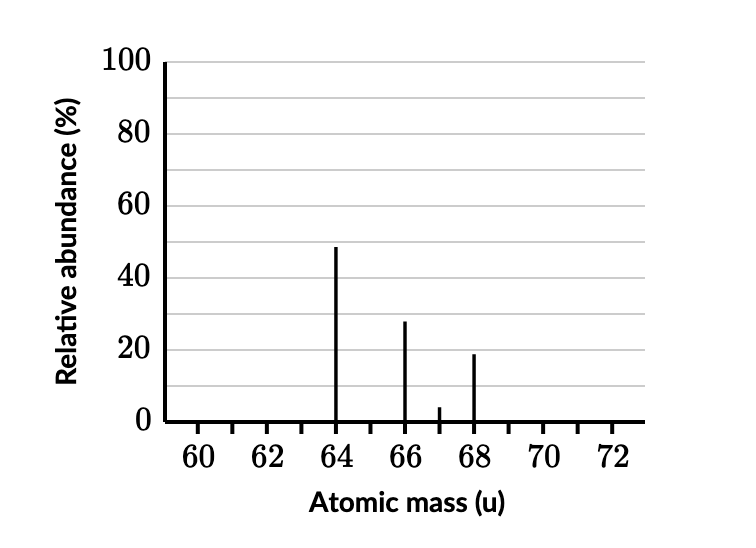
\includegraphics[scale = 0.5]{photo1.png}
\end{center}
(a) In an average sample of the element, less than \(20\%\) of the atoms have an atomic mass of \(66u\). \\
(b) The most abundant isotope of the element has an atomic mass of \(64u\). \\
(c) The element has an average atomic mass of \(64u\). \\
(d) The element has an average atomic mass between \(66\) and \(68u\). \\
\subsection*{Problem \countThis}
What is the percent composition of Carbon in \(\ce{C_{13}H_{18}O_2}\)?
\subsection*{Problem \countThis}
A compound contains \(32.38\%\) sodium, \(22.65\%\) sulfur, and \(44.99\%\) oxygen. What is the emperical forumula. 
\subsection*{Problem \countThis}
What is the full electron configuration of mercury?
\subsection*{Problem \countThis}
Below, the photoelectron spectra of the \(2s\) electrons of \(\ce{Be}\) and \(\ce{Mg}\) are shown.
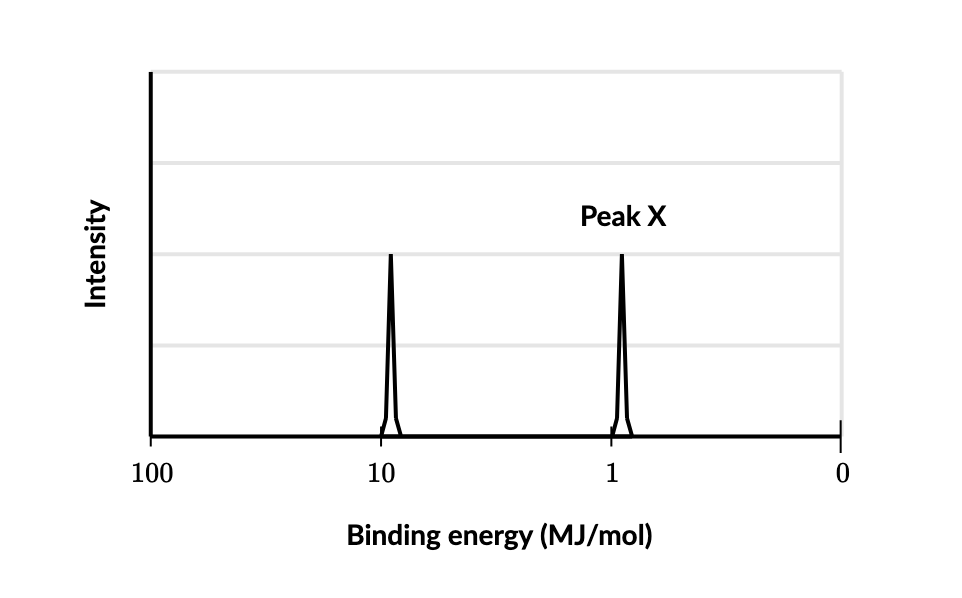
\includegraphics[scale = 0.5]{photo2.png} \\
Is peak \(X\) the peak associated with \(\ce{Be}\) or \(\ce{Mg}\)?
\subsection*{Problem \countThis}
What are the periodic trends of ionization energy, atomic radius, and electronegativity? Why?
\section{Unit 2: Molecular and Ionic Compound Structure and Properties}
\subsection*{Problem \countThis}
Which of the following bonds is likely to have the most ionic character? \\
(a) \chemfig{H-F} \\
(b) \chemfig{C-O} \\
(c) \chemfig{Na-F}\\
(d) \chemfig{Mg-O}
\subsection*{Problem \countThis}
Based on the information in the table, which of the following arranges the bonds in order of decreasing polarity? \\
\begin{center}
\begin{tabular}{|cc|}
    \hline 
    Element & Electronegativity \\ [0.5 ex]
    \hline \hline
    \(\ce{H}\) & \(2.2\)\\
    \(\ce{N}\) & \(3.0\) \\
    \(\ce{F}\) & \(4.0\) \\
    \(\ce{Cl}\) & \(3.2\) \\
    \(\ce{Se}\) & \(2.6\) \\
    \(\ce{I}\) & \(2.7\)\\ [1ex]
    \hline
\end{tabular}
\end{center} 
(a) \(\chemfig{Se-N} > \chemfig{H-I} > \chemfig{Cl-F}\) \\
(b) \(\chemfig{H-I} > \chemfig{Se-N} >\chemfig{Cl-F}\)\\
(c) \(\chemfig{Cl-F} > \chemfig{H-I} > \chemfig{Se-N}\)\\
(d) \(\chemfig{Cl-F} > \chemfig{Se-N} > \chemfig{H-I}\)
\subsection*{Problem \countThis}
Why is the lattice energy of \ce{CsF} smaller than the lattice energy of \ce{KF}?
\subsection*{Problem \countThis}
What type of structure do metallic elements form and through what bonds? 
\subsection*{Problem \countThis}
What are the two types of metallic alloys and what are there differences?
\subsection*{Problem \countThis}
Draw a Lewis Diagram for Acetic Acid \ce{CH3COOH}.
\subsection*{Problem \countThis}
Draw the Lewis Diagram for \ce{CO2}
\subsection*{Problem \countThis}
Draw the Lewis Diagram(s) for ozone, \ce{O3}
\ProblemSet
Write the formal charges for all three molecules above.
\ProblemSet
What is the electron geometry, molecular geometry, and hybridization of the central atom in this molecule. \\ 
\chemfig{\charge{-90=\:}{N}(-[:90]H)(-[:225]H)(-[:315]H)}
\section{Unit 3: Intermolecular Forces and Properties}
\ProblemSet
What are the intermolecular forces present among these molecules. \\ 
\chemfig{H-C(-[:-90]H)(-[:90]H)-C(=[:90]O)-O-C(-[:90]H)(-[:-90]H)-H}
\ProblemSet
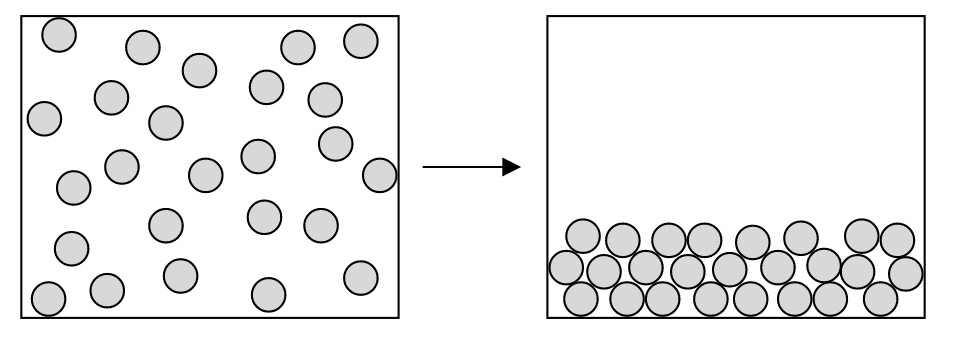
\includegraphics[scale = 0.5]{photo3.png} \\
What phase transition is this?
\ProblemSet
Originally, a sample of gas is in a rigid container at \(299K\) and \(0.70 atm\). The student increases the temperature of the \ce{CO2(g)} in the container to \(425K\).\\
(a) What does raising the temperature do to the motion of the molecules?\\
(b) What is the pressure at \(425K\)?\\
(c) In terms of Kinetic Molecular Theory, why does the pressure of gas change as it is heated? \\
\ProblemSet
A \(60.3g\) of \ce{Be(OH)2} is dissolved in enough water to produce \(1.75L\) of solution. Calculate the concentration of \ce{OH-} ions. 
\ProblemSet
Describe the photoelectric effect. 
\ProblemSet
List \ce{HCOOH}, \ce{H2S}, and \ce{Ar} in order of increasing intermolecular forces. 
\ProblemSet
What are the intermolecular forces for this molecule:\\
\chemfig{C*6((-H)-C(-H)=C(-H)-C(-H)=C(-H)-C(-H)=)} 
\ProblemSet
Which of the following will require the greatest energy input to separate the ions?\\
(a) \ce{MgI2}\\
(b) \ce{MgF2}\\
(c) \ce{MgCl2}\\
(d) \ce{MgBr2}\\
\ProblemSet
Why does \ce{I2} have a higher boiling point than \ce{Cl2}?
\ProblemSet
Is \ce{CO2} polar? Why?
\section{Unit 4: Chemical Reactions}
\ProblemSet
Balance this reaction:
\ce{C5H_{10} + O2 -> CO2 + H2O}
\ProblemSet
Balance this redox reaction: \ce{MnO4- + I- -> I2 + Mn^{2+}}
\ProblemSet
Aqueous \ce{FeCl3} reacts with \ce{KOH} to produce a solid precipitate of \ce{Fe(OH)3} and aqueous \ce{KCl}. What is the balanced net ionic equation? 
\ProblemSet
What is the difference between physical changes and chemical changes?
\ProblemSet
\ce{H2O} and \ce{Fe} are reacted according to the reaction below. There was initially \(36.0g\) \ce{H2O} and \(67.0g\) \ce{Fe}. What is the limiting reactant, how much of the excess reactant will remain, and how much iron oxide is produced? \\
\ce{3Fe(s) + 4H2O(g) -> Fe3O4(s) 4H2(g)}
\ProblemSet
A \(56kg\) sample of \ce{CO} and \(6.0kg\) sample of \ce{H2} are combined into a closed vessel. \\
\ce{CO(g) + 2H2(g) ->CH3OH(g) } \\
How many moles of \ce{CH3OH(g)} have been produced?
\ProblemSet
Balance this reaction: \\
\ce{Al(s) + O2(g) -> Al2O3} 
\ProblemSet
Balance this reaction:\\
\ce{V + O2 -> V2O5}
\ProblemSet
Balance this reaction: \\
\ce{C6H_{12}O6 + O2 -> CO2 + H2O}
\ProblemSet
Balance this reaction: \\
\ce{Mg + O2 -> MgO}
\section{Unit 5: Kinetics}
\ProblemSet
For this reaction: \\
\ce{CH4(g) + 2O2(g) -> CO2(g) + 2H2O(g)} \\
What would be rate be in terms of each reactant and product. \\
\ce{CH4} \hspace{0.5em} rate = \\
\ce{O2} \hspace{0.5em} rate = \\
\ce{CO2} \hspace{0.5em} rate = \\
\ce{H2O} \hspace{0.5em} rate = 
\ProblemSet
If the rate of dissapearance of \ce{CH4} equals \(5.0\frac{M}{s}\) for the above reaction, what is the rate of appearance of \ce{H2O}?
\ProblemSet
For the above reaction, what is the reaction rate if \ce{O2} decreases from \(0.1M\) to \(0.04M\) in \(125ms\)?
\ProblemSet
\ce{A(aq) + 2B(aq) -> Products}
\begin{center}
    \begin{tabular}{||c c c c||} 
     \hline
     Experiment & \([A]_0\) & \([B]_0\) & Initial Rate \\ [0.5ex] 
     \hline\hline
     1 & \(0.10M\) & \(0.10M\) & \(1.0 \times 10^{-2}\frac{M}{s}\) \\ [1ex]
     \hline
     2 & \(0.3M\) & \(0.10M\) & \(9.0 \times 10^{-2}\frac{M}{s}\) \\[1ex]
     \hline
     3 & \(0.3M\) & \(0.15M\) & \(9.0 \times 10^{-2} \frac{M}{s}\) \\ [1ex] 
     \hline
    \end{tabular}
\end{center}
What is the rate law?
\ProblemSet
\ce{N2O5} decomposes by a 1st order reaction with \(k = 4.80 \times 10^{-4} \frac{1}{s}\). What is the concentration of \ce{N2O5} after \(825\) seconds if the 
intial concentration is \(0.0165M\)? What is the half-life for this reaction?
\ProblemSet
\textbf{This problem relates to problem \theyayCounter{} as well }\\
The reaction \ce{2C4H6(g) -> C8H_{12}(g)} is a 2nd order reaction with \(k = 4.0 \times 10^{-4}\frac{1}{Ms}\). If the initial concentration of \ce{C4H6} is
\(0.100M\) what is the concentration after 6 days?
\ProblemSet
How long does it take for the concentration to drop to \(0.085M\)?
\ProblemSet
What is the net chemical reaction and predict the experimental rate law for a chemical reaction with this chemical mechanism.
\begin{equation*}
    \begin{aligned}
        &\ce{H2O2 + I- ->H2O + IO-} \hspace{1em} k_1 \hspace{0.1em} \text{(slow)} \\
        &\ce{IO- + H2O2 -> H2O + O2 + I-} \hspace{1em} k_2 \hspace{0.1em} \text{(fast)}
    \end{aligned}
\end{equation*}
Also identify catalysts and intermediates.
\ProblemSet
Predict the experimental rate law for a chemical reaction that proceeds by the following mechanism:
\begin{equation*}
    \begin{aligned}
        & \ce{2NO <=> N2O2} \hspace{1em} \text{(Fast equilibrium step)} \\
        & \ce{N2O2 + H2 -> H2O + N2O} \hspace{1em} \text{(slow)} \\
        & \ce{N2O + H2 -> N2 + H2O} \hspace{1em} \text{(fast)} 
    \end{aligned}
\end{equation*}
\section{Unit 6: Thermodynamics}
\ProblemSet
It takes \(1.8\times 10^{-19}\) calories of energy to break an \chemfig{O-H} bond in water. How much energy does it take to break all of the \chemfig{O-H}
bonds in \(50.0\) grams of water?
\ProblemSet
\(120.\) grams of an unknown metal at \(100.\degree C\) is dropped in a styrofoam cup  that contains \(100.0mL\) of water that is at \(20.0\deg C\). After some times,
the final temperature of the equilibiated system is measured to be \(27.3\degree C\). What is the specific heat capacity of the metal?
\ProblemSet
How much heat energy is required to vaporize \(5.0\) liters of \ce{H2O(l)} where the heat of vaporization of water is \(40.72\frac{kJ}{mol}\).
\ProblemSet
Given these chemical equations \\
\ce{C2H2(g) + 2H2(g) -> C2H6(g)} \hspace{1em} \(\Delta H = -311kJ\) \\
\ce{C2H4(g) + H2(g) -> C2H6(g)} \hspace{1em} \(\Delta H = -136kJ\) \\
Find the enthalpy change for \\
\ce{C2H2(g) + H2(g) -> C2H6(g)}
\ProblemSet
For \ce{C2H5OH(l) + 2O2(g) -> 2CO2(g) + 2H2O(l)} \hspace{1em} \(\Delta H = -1371kJ\). If \(1.5mol\) of oxygen is used, how much energy is released?
\ProblemSet
When temperature increases, does entropy increase or decrease?
\ProblemSet
If the standard entropies for \ce{H2O(g)}, \ce{H2(g)}, and \ce{O2} are \(188.83\), \(130.58\), and \(205.0\) respectively, what is the entropy change for \ce{2H2O(g) -> 2H2(g) + O2(g)}? 
\ProblemSet
What is \(\Delta S_{universe}\) for the equation \ce{CH4(g) + 2O2(g) <=> CO2(g) + 2H2O(g)} where \(\Delta H = -802.2\frac{kJ}{mol}\). Use the standard entropy values above and note that \(S\degree = 213.7\) and \(186.1\) for \ce{CO2(g)} and \ce{CH4(g)} respectively. 
\ProblemSet
For \ce{N2(g) + 2H2(g) <=> 2NH3(g)} where \(\Delta H = -91.8 kJ\) and \(\Delta S\degree = -197.3\frac{J}{K}\). Calculate \(\Delta G\degree\) at \(1000K\)
\ProblemSet
For \ce{2H2O(g) <=> 2H2(g) + O2(g)} \hspace{1em} \(\Delta H\degree = 483.6kJ\). Will the reaction form more or less product when temperature is increased. 
\section{Unit 7: Equilibrium}
\ProblemSet
What is the concentration equilibrium constant for the reaction \ce{CO(g) + 3H2(g) <=> CH4(g) + H2O(g)}
\ProblemSet
If \(K_c = 3.91\) at \(1200K\), Will the reactants shift towards products, reactants, or stay the same if the reaction mixture contains \([\ce{CO}] = 0.0200M\), \([\ce{H2}] = 0.0200M\), \([\ce{CH4}] = 0.00100M\), and \([\ce{H2O}] = 0.00100M\)?
\ProblemSet 
For this chemical reaction \ce{2CH4(g) <=> C2H2(g) + 3H2(g)}, \(K_p = 2.0\times 10^{-6}\). \(14 atm\) of methane gas is put into the reaction vessel. What is the expected partial pressure of \ce{C2H2(g)} at equilibrium. 
\ProblemSet
For this reaction \ce{NH4HS(s) <=> NH3(g) + H2S(g)}, \(K_c = 0.16\). What is the molar concentration of each product if \(250g\) of ammonium hydrogen sulfide is introduced into a \(2.0L\) flask and allowed to reach equilibrium. 
\ProblemSet
What is the molar solubility of \ce{AgCl} in water at \(24\degree C\) where \(K_{sp} = 1.8 \times 10^{-10}\) for \ce{AgCl} at this temperature.
\ProblemSet 
What is the solubility of \ce{Ca3(PO4)2} in water at \(25\degree C\) in where \(K_{sp} = 1.2\times 10^{-29}\). 
\ProblemSet
\(15mg\) of \ce{CaF2} dissolves in \(1.00L\) of water at \(25\degree C\). What is \(K_{sp}\) for \ce{CaF2} at this temperature?
\ProblemSet 
What is the molar concentration of \ce{OH-} in an aqueous \(1.3M\) \ce{HCl} solution at \(24\degree C\)?
\ProblemSet
What is the pH of an aqueous solution of \(0.050M\) \ce{HNO3} solution at \(25\degree C\)?
\ProblemSet
What is the pH of a weak acid with a \(K_a = 2.6\times 10^{-5}\)? 
\section{Unit 8: Acids and Bases}
\ProblemSet
Calculate the pH of  a solution that is \(0.5M\) \ce{CH3COOH} and \(0.10M\) \ce{KCH3COO}.
\ProblemSet
Calculate the pH of a solution that is \(0.10M\) \ce{CH3COOH} and \(0.50M\) \ce{KCH3COO}.
\ProblemSet
Which of the following buffer systems would be the best choice for preparing a \(pH = 4.10\) buffer solution.\\ 
(a) \ce{HNO2}/\ce{NaNO2} \hspace{1em} \(K_a = 7.1\times 10^{-4}\) \\
(b) \ce{HCOOH}/\ce{KHCOO}\hspace{1em}\(K_a = 1.8\times 10^{-4}\)\\
(b) \ce{C6H5COOH}/\ce{NaC6H5COO}\hspace{1em}\(K_a = 6.3\times 10^{-5}\)\\
\ProblemSet
Will \(0.2mol\ce{NH3}\) and \(0.2mol\ce{NH4Cl}\) be a buffer solution? 
\ProblemSet
Will \(0.2mol\ce{CH3COOH}\) and \(0.1mol\ce{NaOH}\) be a buffer solution?
\ProblemSet
A \(0.10M\) weak acid solution has a \(pH = 3.7\). What is the percent ionization of the acid in this solution? 
\ProblemSet
Why is \ce{HF} weak but \ce{HCl} is  a strong acid?
\ProblemSet
Why is \ce{HClO4} a strong acid but \ce{HClO2} a weak acid? 
\ProblemSet
What is the conjugate base of \ce{HSO4-}?
\ProblemSet
What is the concentration of the hydroxide ion in pure water at \(25\degree C\)?
\section{Unit 9: Applications of Thermodynamics}
\ProblemSet
For this reaction, which element is oxidized or reduced at the anode.\\
\ce{2NaCl(l) -> 2Na(l) + Cl2(g)}
\ProblemSet
For the reaction \(\ce{2Al^{3+}(aq) + 3Mg(s) -> 2Al(s) + 3Mg^{2+}(aq)}\). What are the half reactions?
\ProblemSet
Using the chemical reaction above:\\
If \(E\degree =0.71V\) what is the cell potential if all the reactants are in their standard states except \(\ce{Al^{3+}}\) which is present at \(0.010M\)?
\ProblemSet
Using the chemical reaction above:\\
What is the change in mass of the alumnimum electrode if this cell discharges for \(100.0s\) with a current of \(0.1A\)?

\end{document}
